\chapter{Từ nam châm Ising đến tính tới hạn lỏng--khí}

\lectureoverview{Chuyển pha lỏng--khí có thể được tiếp cận theo một con đường bất ngờ. Trước hết, ta hoàn tất cách xử lý trường trung bình của nam châm Ising, xác định đường cùng tồn tại và điểm tới hạn của nó, rồi diễn giải lại một spin hướng lên như một nút mạng được chiếm. Khí mạng thu được có loại trừ lõi cứng, lực hút tầm ngắn, một thế hóa học do từ trường điều khiển, và giản đồ pha hoàn toàn giống hệt. Phần bài giảng chính thức kết thúc bằng hành vi tới hạn và tính phổ quát. Sau đó, một phần thảo luận riêng sau bài giảng khảo sát điều mà các nhà vật lý muốn nói khi nhắc đến sự tinh chỉnh, cách các hiệu ứng chọn lọc có thể đi vào một lời giải thích, và vì sao kiểu lập luận ấy chỉ hữu ích khi gắn với một cơ chế và các phép kiểm nghiệm khả dĩ.}

\section{Vì sao nước sôi lại bắt đầu từ một nam châm}

Nước sôi là hiện tượng quen thuộc mà ta muốn hiểu: một chất lỏng chuyển thành chất khí và mật độ của nó thay đổi đột ngột. Con đường tiêu chuẩn đi qua phương trình van der Waals. Ở đây ta đi theo một con đường khác. Ta quay lại nam châm Ising, hoàn tất mô tả trường trung bình của nó, rồi nhận ra rằng cùng một mô hình ấy có thể được hiểu như một chất lưu.

Đây không chỉ là một phép tương tự gợi hình. Một khi các biến đã được chuyển đổi đúng cách, nam châm Ising và khí mạng là cùng một hệ cơ học thống kê. Độ từ hóa trở thành mật độ hạt, từ trường ngoài trở thành một thế hóa học, và đường cùng tồn tại từ tính trở thành đường cùng tồn tại lỏng--khí. Phép chuyển đổi này giải thích vì sao hai loại vật chất bề ngoài khác nhau lại có thể có cùng hành vi tới hạn.

Trường trung bình sẽ không cho các đáp số số trị chính xác ở số chiều thấp. Trong một chiều, nó thậm chí còn dự đoán một chuyển pha mà nghiệm đúng không cho phép. Giá trị của nó ở đây nằm ở cấu trúc. Trong hai và ba chiều, nó làm lộ ra đúng tham số trật tự, các pha cạnh tranh, đầu mút tới hạn, và cách một thiên lệch vô cùng nhỏ chọn ra một pha. Trong ba chiều, nơi mỗi nút có sáu láng giềng gần nhất, việc thay các láng giềng đó bằng giá trị trung bình của chúng đã cho một bức tranh định tính hữu ích.

\section{Hạch toán năng lượng của Ising}

Đặt một spin hai trạng thái tại mỗi nút của một mạng siêu lập phương,
\begin{equation}
\sigma_i=\pm1.
\end{equation}
Ta dùng Hamiltonian
\begin{equation}
\mathcal H
=-J\sum_{\langle ij\rangle}\sigma_i\sigma_j
+h\sum_i\sigma_i,
\qquad J>0.
\label{eq:ising-hamiltonian}
\end{equation}
Ký hiệu ở đây rất quan trọng. Tổng thứ nhất chạy trên các \emph{liên kết} giữa các láng giềng gần nhất; tổng thứ hai chạy trên các \emph{nút mạng}. Mỗi liên kết chỉ được đếm một lần, không phải một lần từ mỗi đầu mút.

Với một liên kết đơn lẻ,
\begin{equation}
E_{ij}=-J\sigma_i\sigma_j.
\end{equation}
Các spin song song có năng lượng \(-J\), còn các spin đối song song có năng lượng \(+J\). Vì vậy, một liên kết bị gãy tốn
\begin{equation}
\Delta E_{\rm bond}=+J-(-J)=2J.
\label{eq:broken-bond}
\end{equation}
Đại lượng \(2J\), chứ không phải một trong hai năng lượng liên kết tuyệt đối, mới là thứ chi phối các trọng số Boltzmann tương đối. Ta có thể cộng thêm một hằng số vào mọi cấu hình mà không làm thay đổi bất kỳ xác suất nào.

\begin{classroomqa}
\audiencequestion{Vì sao trong Hamiltonian lại có hai phép tổng khác nhau?}
\lecturerresponse{Năng lượng trao đổi gắn với một cặp nút lân cận, nên nó được lấy tổng trên các liên kết \(\langle ij\rangle\). Trường tác dụng độc lập lên từng spin, nên nó được lấy tổng trên các nút \(i\). Nhầm lẫn hai cách đếm ấy sẽ đưa vào đúng những hệ số 2 sẽ trở nên quan trọng trong trường trung bình. \lecturetimestamp{00:08:04--00:08:45}}
\end{classroomqa}

\begin{classroomqa}
\audiencequestion{Việc làm \(J\) lớn hơn có đơn giản chỉ khiến mọi năng lượng trở nên âm hơn không?}
\lecturerresponse{Nó làm tăng độ chênh lệch giữa các cấu hình đồng hướng và nghịch hướng. Mốc không của năng lượng là tùy ý; phát biểu vật lý ở đây là một liên kết bị gãy tốn \(2J\). Vì thế \(J\) dương lớn hơn làm cho sự mất trật tự nhiệt kém thuận lợi hơn ở một nhiệt độ cố định. \lecturetimestamp{00:08:47--00:10:17}}
\end{classroomqa}

Trên một mạng siêu lập phương vô hạn hoặc tuần hoàn trong \(d\) chiều, mỗi nút có \(2d\) láng giềng. Đếm từ toàn bộ \(N\) nút sẽ đếm mỗi liên kết hai lần, nên
\begin{equation}
N_{\rm links}=\frac{(2d)N}{2}=dN.
\label{eq:number-links}
\end{equation}
Do đó một cấu hình đồng hướng có năng lượng trao đổi \(-JdN\). Các nút biên làm thay đổi kết quả này bởi một số hạng bề mặt, không đáng kể so với \(N\) trong giới hạn nhiệt động. Hai trạng thái hoàn toàn đồng hướng là suy biến khi \(h=0\).

Số hạng trường ấn định một quy ước dấu mà ta sẽ giữ nhất quán. Trong phương trình~\eqref{eq:ising-hamiltonian}, giá trị dương của \(h\) cho \(\sigma=-1\) năng lượng nút thấp hơn. Do đó \(h>0\) ưu tiên độ từ hóa âm, còn \(h<0\) ưu tiên độ từ hóa dương. Có thể đảo quy ước này bằng cách viết \(-h\sum_i\sigma_i\); không có gì vật lý thay đổi, nhưng khi đó mọi dấu về sau cũng phải đảo theo.

\begin{classroomqa}
\audiencequestion{Nhiệt độ đi vào ở đâu nếu Hamiltonian chỉ chứa \(J\) và \(h\)?}
\lecturerresponse{Nhiệt độ đi vào qua thừa số Boltzmann \(e^{-\beta\mathcal H}\), với \(\beta=1/T\) trong đơn vị \(k_{\rm B}=1\). Vì thế các đại lượng không thứ nguyên là \(\beta J\) và \(\beta h\). \lecturetimestamp{00:13:07--00:13:43}}
\end{classroomqa}

\section{Một spin trong trường trung bình của các láng giềng của nó}

Chọn một spin ở xa biên. Nó có \(2d\) láng giềng gần nhất. Trong trường trung bình, mỗi láng giềng dao động được thay bằng cùng một giá trị trung bình
\begin{equation}
m=\expect{\sigma}.
\end{equation}
Khi đó năng lượng trao đổi có chứa spin được chọn \(\sigma\) là
\begin{equation}
-J\sigma\sum_{\text{\(2d\) neighbors}}\sigma_j
\;\longrightarrow\;-2dJm\,\sigma.
\end{equation}
Cộng thêm trường ngoài cho ta năng lượng hữu hiệu của một spin
\begin{equation}
\mathcal H_{\rm mf}(\sigma)=(-2dJm+h)\sigma.
\label{eq:mean-field-one-spin}
\end{equation}
Hệ số \(2d\) là thiết yếu. Rất dễ bỏ sót nó khi viết bức tranh spin trung tâm, và nó đã được đưa trở lại một cách tường minh trong phép suy ra trên bảng.

\begin{figure}[ht]
\centering
\includegraphics[width=0.84\textwidth]{lecture_10_figure_02.png}
\caption{Một spin trung tâm được bao quanh bởi các láng giềng trường trung bình của nó, cùng với năng lượng một spin và phương trình tự nhất quán đang được thiết lập.}
\lectureframe{00:17:57}
\end{figure}

Hàm phân hoạch một spin là
\begin{align}
z_{\rm mf}
&=\sum_{\sigma=\pm1}
\exp\!\left[-\beta(-2dJm+h)\sigma\right] \\
&=2\cosh\!\left[\beta(2dJm-h)\right].
\end{align}
Spin trung bình của nó là
\begin{align}
\expect{\sigma}
&=\frac{\sum_{\sigma=\pm1}\sigma
 e^{\beta(2dJm-h)\sigma}}
{\sum_{\sigma=\pm1}e^{\beta(2dJm-h)\sigma}} \\
&=\tanh\!\left[\beta(2dJm-h)\right].
\end{align}
Nhưng spin ta chọn được giả định là điển hình cho các láng giềng mà giá trị trung bình của chúng ta gọi là \(m\). Vì thế điều kiện tự nhất quán là
\begin{equation}
\boxed{m=\tanh\!\left[\beta(2dJm-h)\right].}
\label{eq:mean-field-self-consistency}
\end{equation}
Phương trình phi tuyến duy nhất này là sự rút gọn trường trung bình của bài toán nhiều spin.

\begin{classroomqa}
\audiencequestion{Vì sao giá trị trung bình ở vế trái lại chính là cùng \(m\) đã được đưa vào cho mọi láng giềng?}
\lecturerresponse{Sự đồng nhất ấy chính là phép gần đúng. Ta giả sử một trạng thái khối đồng nhất, thay môi trường thực sự bằng giá trị trung bình của nó, tính spin trung tâm trong môi trường đó, rồi đòi hỏi rằng giá trị trung bình tính được phải tái tạo lại môi trường mà ta đã giả định. Một nghiệm là một trạng thái khối tự nhất quán. \lecturetimestamp{00:16:28--00:18:00}}
\end{classroomqa}

Đặt
\begin{equation}
y=2\beta dJm.
\label{eq:y-definition}
\end{equation}
Vì \(\beta=1/T\),
\begin{equation}
m=\frac{yT}{2dJ},
\end{equation}
và phương trình~\eqref{eq:mean-field-self-consistency} trở thành
\begin{equation}
\boxed{\frac{yT}{2dJ}=\tanh(y-\beta h).}
\label{eq:reduced-mean-field}
\end{equation}

\begin{figure}[ht]
\centering
\includegraphics[width=0.82\textwidth]{lecture_10_figure_03.png}
\caption{Phương trình tự nhất quán rút gọn sau khi đưa vào \(y=2\beta dJm\), sẵn sàng để giải bằng đồ thị.}
\lectureframe{00:24:42}
\end{figure}

\begin{classroomqa}
\audiencequestion{Vì sao trường xuất hiện dưới dạng \(y-\beta h\), và trường dương ưu tiên spin nào?}
\lecturerresponse{Hamiltonian của ta chứa \(+h\sigma\). Vì thế số mũ Boltzmann của nó là \(\beta(2dJm-h)\sigma\), nên hàm tang hyperbol chứa \(y-\beta h\). \(h\) dương ưu tiên \(\sigma=-1\). Nếu thay vào đó ta định nghĩa Hamiltonian với \(-h\sigma\), thì mọi chỗ xuất hiện của \(h\) đều đổi dấu và giản đồ pha bị phản chiếu theo phương ngang. \lecturetimestamp{00:18:17--00:20:00}}
\end{classroomqa}

\section{Nghiệm đồ thị và điểm Curie}

Đặt \(h=0\). Ta phải tìm các giao điểm của
\begin{equation}
\frac{T}{2dJ}y
\qquad\text{and}\qquad
\tanh y.
\end{equation}
Đường thứ nhất là một đường thẳng đi qua gốc tọa độ; đường thứ hai là một đường cong lẻ, bão hòa. Ở nhiệt độ cao, đường thẳng dốc và giao điểm duy nhất là \(y=0\), do đó \(m=0\). Khi nhiệt độ hạ xuống, đường thẳng trở nên thoải hơn. Nhiệt độ tới hạn đạt được khi đường thẳng và hàm tang hyperbol tiếp xúc nhau tại gốc tọa độ.

\begin{figure}[ht]
\centering
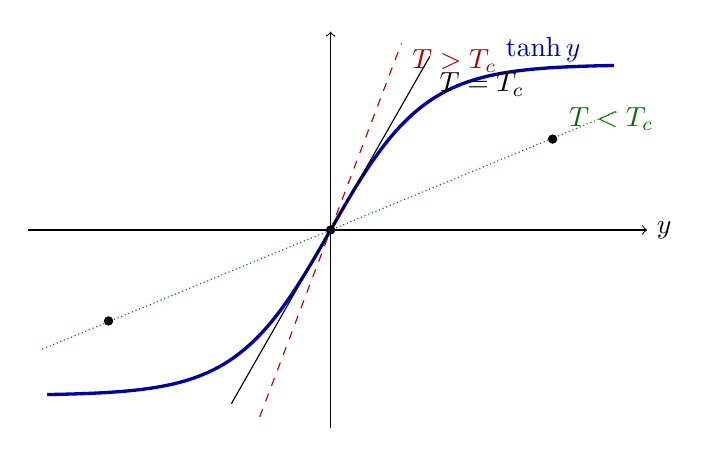
\begin{tikzpicture}[x=1.2cm,y=2.1cm]
\draw[->] (-3.2,0) -- (3.35,0) node[right] {$y$};
\draw[->] (0,-1.2) -- (0,1.2);
\draw[very thick,blue!65!black,domain=-3:3,samples=120]
  plot (\x,{tanh(\x)});
\node[blue!65!black,above] at (2.25,0.96) {$\tanh y$};
\draw[dashed,red!70!black] (-0.75,-1.13) -- (0.75,1.13);
\node[red!70!black,right] at (0.76,1.02) {$T>T_c$};
\draw[black] (-1.05,-1.05) -- (1.05,1.05);
\node[right] at (1.05,0.88) {$T=T_c$};
\draw[densely dotted,green!45!black] (-3.05,-0.72) -- (3.05,0.72);
\node[green!45!black,right] at (2.42,0.67) {$T<T_c$};
\fill (-2.35,-0.55) circle (1.7pt);
\fill (0,0) circle (1.7pt);
\fill (2.35,0.55) circle (1.7pt);
\end{tikzpicture}
\caption{Phương trình trường trung bình ở trường bằng không. Dưới \(T_c\), hai giao điểm khác không biểu diễn các pha từ hóa ổn định; nghiệm không vẫn còn hiện diện về mặt đại số nhưng không ổn định.}
\label{fig:mean-field-intersections}
\end{figure}

Do
\begin{equation}
\left.\frac{d}{dy}\tanh y\right|_{y=0}=1,
\end{equation}
điều kiện tiếp xúc là
\begin{equation}
\frac{T_c}{2dJ}=1.
\end{equation}
Vì thế trường trung bình dự đoán
\begin{equation}
\boxed{T_c^{\rm MF}=2dJ.}
\label{eq:sm10-mean-field-tc}
\end{equation}
Bên dưới nhiệt độ này có hai nghiệm ổn định khác không \(\pm m_0(T)\). Nghiệm \(m=0\) vẫn thỏa mãn phương trình, nhưng nó không còn là cân bằng ổn định nữa. Hệ chọn một trong hai pha từ hóa liên hệ với nhau bởi đối xứng.

\begin{classroomqa}
\audiencequestion{Đây có phải là nhiệt độ Curie không?}
\lecturerresponse{Đúng. Với một nam châm sắt từ, nhiệt độ tại đó độ từ hóa tự phát biến mất theo quy ước được gọi là nhiệt độ Curie. Ở đây \(2dJ\) là giá trị trường trung bình của nó, không phải một kết quả đúng chính xác trong số chiều thấp. \lecturetimestamp{00:28:19--00:28:57}}
\end{classroomqa}

Gần chuyển pha, khai triển hàm tang hyperbol:
\begin{equation}
\tanh y=y-\frac{y^3}{3}+O(y^5).
\end{equation}
Tại \(h=0\), phương trình~\eqref{eq:reduced-mean-field} cho
\begin{equation}
\left(1-\frac{T}{T_c}\right)y-\frac{y^3}{3}+O(y^5)=0.
\end{equation}
Vì thế các nhánh khác không có dạng
\begin{equation}
y^2\simeq3\left(1-\frac{T}{T_c}\right),
\qquad
m\propto(T_c-T)^{1/2}.
\label{eq:mf-beta-exponent}
\end{equation}
Dạng căn bậc hai này tương ứng với một số mũ tới hạn của trường trung bình. Giá trị chính xác của số mũ ấy sẽ không còn đúng trong số chiều thấp, nhưng sự biến mất liên tục của tham số trật tự tại đầu mút thì vẫn còn.

\section{Mặt phẳng nhiệt độ--trường và sự chọn nhánh}

Vật liệu xác định \(J\); người làm thí nghiệm có thể thay đổi \(T\) và \(h\). Vì thế, tự nhiên là ta vẽ một giản đồ pha trong mặt phẳng \(T\)--\(h\). Bên dưới \(T_c\), một trường nhỏ đến tùy ý cũng đủ để chọn một trong hai nhánh từ hóa. Theo quy ước của chúng ta, \(h<0\) chọn \(m>0\), còn \(h>0\) chọn \(m<0\).

Ở nhiệt độ bằng 0, các spin thẳng hàng hoàn toàn, nên \(m=\pm1\). Ở nhiệt độ cao, giá trị trung bình khi không có trường là \(m=0\). Khi tiến tới điểm tới hạn dọc theo \(h=0\), độ lớn \(m_0(T)\) giảm liên tục về 0. Nhưng với bất kỳ \(T<T_c\) cố định nào, việc đi qua \(h=0\) sẽ chuyển gián đoạn từ \(+m_0(T)\) sang \(-m_0(T)\).

\begin{figure}[ht]
\centering
\includegraphics[width=0.90\textwidth]{lecture_10_figure_06.png}
\caption{Đường cùng tồn tại trong mặt phẳng \(T\)--\(h\) và các nhánh từ hóa ở nhiệt độ cố định dưới \(T_c\).}
\lectureframe{00:39:30}
\end{figure}

\begin{figure}[ht]
\centering
\resizebox{\linewidth}{!}{%
\begin{tikzpicture}[x=1.25cm,y=1.15cm]
\begin{scope}
\draw[->] (-2.45,0) -- (2.55,0) node[right] {$h$};
\draw[->] (0,0) -- (0,3.7) node[above] {$T$};
\draw[very thick,red!70!black] (0,0) -- (0,2.35);
\fill[red!70!black] (0,2.35) circle (2.3pt);
\node[right] at (0.08,2.35) {$T_c$};
\node at (-1.25,1.05) {$m>0$};
\node at (1.25,1.05) {$m<0$};
\draw[->,rounded corners,blue!65!black] (-1.65,0.85) -- (-1.65,3.02)
 -- (1.65,3.02) -- (1.65,0.85);
\node[blue!65!black] at (0,3.35) {continuous path};
\end{scope}
\begin{scope}[xshift=7.0cm,yshift=1.55cm]
\draw[->] (-2.5,0) -- (2.5,0) node[right] {$h$};
\draw[->] (0,-1.35) -- (0,1.4) node[above] {$m$};
\draw[very thick,blue!65!black]
  (-2.2,1.05) .. controls (-0.75,1.03) and (-0.2,0.75) .. (-0.08,0.62);
\draw[very thick,blue!65!black]
  (0.08,-0.62) .. controls (0.2,-0.75) and (0.75,-1.03) .. (2.2,-1.05);
\draw[dashed] (0,0.62) -- (0,-0.62);
\fill (0,0.62) circle (1.8pt);
\fill (0,-0.62) circle (1.8pt);
\node at (0,-1.75) {\(T<T_c\)};
\end{scope}
\end{tikzpicture}
}
\caption{Ở \(T<T_c\) cố định, độ từ hóa nhảy khi đi qua đường cùng tồn tại. Trong mặt phẳng hai tham số đầy đủ, thay vào đó hai pha có thể được nối với nhau một cách liên tục bằng cách đi vòng quanh điểm tới hạn.}
\label{fig:ising-phase-plane}
\end{figure}

\begin{classroomqa}
\audiencequestion{Điều gì xảy ra nếu trường đúng bằng 0 ở dưới \(T_c\)?}
\lecturerresponse{Hệ vô hạn lý tưởng có hai pha thuần hoàn toàn tương đương. Mọi thiên lệch dư vô cùng nhỏ, điều kiện biên, hay dao động gắn với cách chuẩn bị đều chọn một trong hai. Tính gián đoạn nhiệt động học được biểu thị bởi hai giới hạn một phía \(m(T,0^-)=+m_0(T)\) và \(m(T,0^+)=-m_0(T)\) theo quy ước dấu của chúng ta. \lecturetimestamp{00:35:04--00:37:10}}
\end{classroomqa}

\begin{classroomqa}
\audiencequestion{Đây có phải chính là hiện tượng trễ không?}
\lecturerresponse{Hiện tượng trễ liên quan đến tính siêu bền và sự chậm trễ phụ thuộc vào lịch sử khi một hệ thực chuyển từ nhánh này sang nhánh kia. Nó có liên quan, nhưng đòi hỏi động lực học vượt ra ngoài giản đồ pha cân bằng và không được phát triển ở đây. \lecturetimestamp{00:37:11--00:37:20}}
\end{classroomqa}

\begin{classroomqa}
\audiencequestion{Có thể nối pha dương và pha âm mà không đi qua một chỗ gián đoạn không?}
\lecturerresponse{Có. Hãy tăng nhiệt độ lên trên \(T_c\), đổi dấu của trường ở đó, rồi hạ nhiệt độ xuống lại. Đường đi ấy đi vòng quanh điểm cuối và độ từ hóa thay đổi liên tục. Bước nhảy chỉ là không thể tránh khỏi khi ta đi qua \(h=0\) tại \(T<T_c\) cố định. \lecturetimestamp{00:37:20--00:38:15}}
\end{classroomqa}

\begin{classroomqa}
\audiencequestion{Độ từ hóa có tiến về không mỗi khi \(h\) tiến về không không?}
\lecturerresponse{Không, ở một nhiệt độ bất kỳ dưới \(T_c\). Khi đó, các giới hạn một phía đều khác không. Độ từ hóa tự phát chỉ tiến về không khi tiến tới chính nhiệt độ tới hạn. \lecturetimestamp{00:38:29--00:39:45}}
\end{classroomqa}

\section{Hộp thấm và thế hóa học}

Giờ ta rời nam châm và bắt đầu lại với các hạt. Hãy hình dung một vùng có thế năng thấp hơn không gian xung quanh. Các vách là thấm: hạt có thể đi vào và đi ra. Nếu năng lượng bên trong thấp hơn một lượng \(\mu\), thì sự chiếm chỗ ở bên trong nhận được hệ số Boltzmann tương đối \(e^{\beta\mu}\). Làm giếng sâu thêm hoặc nâng nó lên sẽ làm thay đổi số hạt trung bình trong hộp.

\begin{figure}[ht]
\centering
\includegraphics[width=0.84\textwidth]{lecture_10_figure_07.png}
\caption{Bức tranh giếng thế của một hộp thấm. Độ chênh năng lượng giữa bên trong và bên ngoài chi phối mức ưu tiên để các hạt ở trong hộp.}
\lectureframe{00:41:30}
\end{figure}

\begin{figure}[ht]
\centering
\resizebox{\linewidth}{!}{%
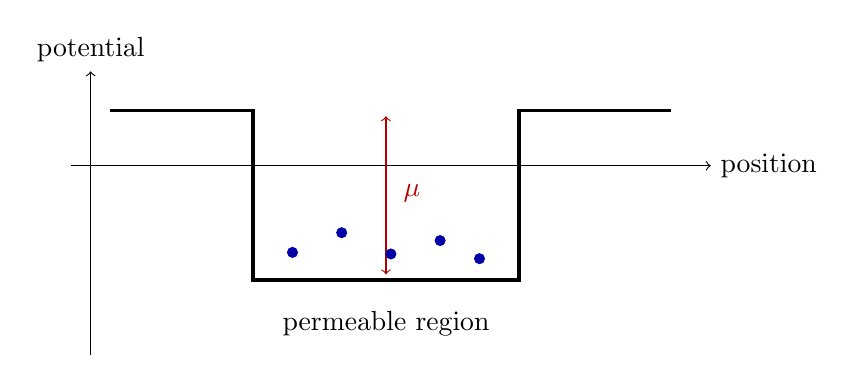
\begin{tikzpicture}[x=1.25cm,y=1.0cm]
\draw[->] (-3.2,0) -- (3.3,0) node[right] {position};
\draw[->] (-3.0,-2.4) -- (-3.0,1.2) node[above] {potential};
\draw[very thick] (-2.8,0.7) -- (-1.35,0.7)
 -- (-1.35,-1.45) -- (1.35,-1.45) -- (1.35,0.7) -- (2.9,0.7);
\draw[<->,red!70!black] (0,0.63) -- (0,-1.38);
\node[right,red!70!black] at (0.08,-0.35) {$\mu$};
\foreach \x/\y in {-0.95/-1.1,-0.45/-0.85,0.05/-1.12,0.55/-0.95,0.95/-1.18}
  \fill[blue!65!black] (\x,\y) circle (2pt);
\node at (0,-2.0) {permeable region};
\end{tikzpicture}
}
\caption{Thay đổi độ dời thế năng làm thay đổi mức ưu tiên về số hạt. Trong mô tả đại chính tắc, độ dời ấy được biểu diễn bằng thế hóa học.}
\end{figure}

Thí nghiệm tư duy này làm cho thế hóa học trở nên cụ thể. Nó là một lợi thế năng lượng cho mỗi hạt được thêm vào so với một bể chứa. Nếu nhiều loại hạt có thể đi qua thành, mỗi loại có thế hóa học riêng. Hộp kín thì khác: khi đó \(N\) được cố định và thế hóa học được suy ra bằng nhiệt động học thay vì được áp đặt bởi sự trao đổi với một bể chứa.

\begin{classroomqa}
\audiencequestion{Độ sâu của giếng có đúng theo nghĩa đen là thế hóa học không?}
\lecturerresponse{Nó là một hiện thực hóa cơ học trực tiếp của một độ chênh thế hóa học. Hạ mọi mức một-hạt ở bên trong xuống \(\mu\) đóng góp \(-\mu N\) vào năng lượng và vì thế đóng góp \(+\beta\mu N\) vào số mũ Boltzmann. Chỉ độ chênh thế hóa học mới quan trọng. \lecturetimestamp{00:44:49--00:45:40}}
\end{classroomqa}

Vì các hạt có thể đi vào và đi ra, tổng phân hoạch phải bao gồm mọi số hạt:
\begin{equation}
\Xi(T,\mu)
=\sum_{N=0}^{\infty}\;\sum_{\mathcal C_N}
\exp\!\left[-\beta E(\mathcal C_N)+\beta\mu N\right].
\label{eq:grand-partition}
\end{equation}
Tổng bên trong chạy trên các cấu hình với \(N\) đã cho; tổng bên ngoài chạy trên chính \(N\). Trọng số đại chính tắc cũng có thể viết là \(e^{-\beta(E-\mu N)}\).

\begin{figure}[ht]
\centering
\includegraphics[width=0.88\textwidth]{lecture_10_figure_08.png}
\caption{Hộp thấm và tổng đại chính tắc trên số hạt và các cấu hình.}
\lectureframe{00:47:15}
\end{figure}

\begin{classroomqa}
\audiencequestion{Điều gì thay đổi khi hộp được bịt kín?}
\lecturerresponse{Số hạt ngừng dao động. Khi đó ta dùng hàm phân hoạch chính tắc tại \(N\) cố định. Trong hộp thấm, \(N\) là một biến nhiệt động được \(\mu\) điều khiển về mặt giá trị trung bình. \lecturetimestamp{00:45:42--00:47:50}}
\end{classroomqa}

Ở nhiệt độ cố định, thay đổi \(\mu\) thường làm mật độ thay đổi trơn. Bên dưới một nhiệt độ tới hạn, thay vào đó nó có thể gây ra một bước nhảy đột ngột. Đó là hiện tượng chất lưu mà ta đang tìm. Để thu được nó ở mức vi mô, các hạt cần có hai đặc trưng: chúng không được có khả năng chiếm cùng một chỗ, và chúng phải hút nhau ở tầm ngắn.

\section{Biến spin thành khí mạng}

Giữ nguyên mạng nhưng diễn giải lại hai trạng thái của nó. Định nghĩa một số chiếm chỗ
\begin{equation}
n_i=\frac{1+\sigma_i}{2}
=
\begin{cases}
0,&\sigma_i=-1,\\
1,&\sigma_i=+1.
\end{cases}
\label{eq:occupation-map}
\end{equation}
Một ô trống có spin xuống; một ô bị chiếm có spin lên. Vì \(n_i\) chỉ có thể bằng 0 hoặc 1, nên bị cấm có hai hạt cùng chiếm một ô. Vì vậy chính bản thân mạng cung cấp lõi cứng.

\begin{figure}[ht]
\centering
\includegraphics[width=0.84\textwidth]{lecture_10_figure_04.png}
\caption{Phép nhận dạng khí mạng bắt đầu bằng việc xem \(\sigma=-1\) là một ô trống; khi đó \(\sigma=+1\) là một ô bị chiếm.}
\lectureframe{00:53:45}
\end{figure}

Xuất phát từ mạng trống, mọi \(\sigma=-1\). Mọi liên kết đều đồng hướng và có năng lượng \(-J\). Năng lượng chân không hằng đó có thể được trừ đi. Bây giờ đặt một hạt lên một ô trong hai chiều. Spin tương ứng lật thành \(+1\), làm gãy bốn liên kết. Mỗi liên kết bị gãy tốn \(2J\), nên
\begin{equation}
\Delta E_1=4(2J)=8J.
\label{eq:one-particle-cost}
\end{equation}
Hai hạt ở xa nhau làm gãy tám liên kết và tốn \(16J\). Nếu hai hạt chiếm các ô lân cận, liên kết giữa chúng lại thẳng hàng. Khi đó chỉ có sáu liên kết biên bị gãy, và chi phí là
\begin{equation}
\Delta E_{2,\rm adjacent}=6(2J)=12J.
\end{equation}
Vì thế đưa các hạt lại gần nhau làm giảm năng lượng một lượng
\begin{equation}
16J-12J=4J.
\label{eq:lattice-attraction}
\end{equation}
Trong phần đếm trực tiếp lúc giảng, ban đầu điều này được mô tả là một khoản tiết kiệm \(2J\) rồi sau đó được sửa lại: một liên kết chung loại bỏ hai đóng góp biên bị gãy, nên lực hút là \(4J\).

\begin{figure}[ht]
\centering
\includegraphics[width=0.84\textwidth]{lecture_10_figure_05.png}
\caption{Phép đếm liên kết trong hai chiều: một hạt cô lập tốn \(8J\), hai hạt ở xa nhau tốn \(16J\), và hai hạt kề nhau tốn \(12J\).}
\lectureframe{01:00:25}
\end{figure}

Khí mạng giờ có cả hai tính chất phân tử cần thiết. Sự chiếm chỗ nhị phân cung cấp sự loại trừ lõi cứng, còn tương tác trao đổi cung cấp lực hút láng giềng gần nhất với cường độ \(4J\). Số hạt được phép dao động vì các phép lật spin làm thay đổi số ô bị chiếm.

\subsection{Phép đối chiếu đại số chính xác}

Bức tranh đếm liên kết là đủ để thấy phần vật lý, nhưng phép đổi biến chính xác làm cho sự tương đương trở nên không thể nhầm lẫn. Thay
\begin{equation}
\sigma_i=2n_i-1
\end{equation}
vào phương trình~\eqref{eq:ising-hamiltonian}. Với một liên kết,
\begin{equation}
\sigma_i\sigma_j
=4n_in_j-2n_i-2n_j+1.
\end{equation}
Trên một mạng đều \(d\) chiều,
\begin{equation}
\sum_{\langle ij\rangle}(n_i+n_j)=2d\sum_i n_i.
\end{equation}
Vì vậy
\begin{align}
\mathcal H
&=-4J\sum_{\langle ij\rangle}n_in_j
+(4dJ+2h)\sum_i n_i+\text{constant}.
\label{eq:ising-as-lattice-gas}
\end{align}
Hãy so sánh điều này với Hamiltonian khí mạng quy ước
\begin{equation}
\mathcal H_{\rm lg}
=-\epsilon\sum_{\langle ij\rangle}n_in_j
-\mu\sum_i n_i+\text{constant}.
\label{eq:lattice-gas-hamiltonian}
\end{equation}
Bảng đối chiếu là
\begin{equation}
\boxed{\epsilon=4J,\qquad
\mu=-(4dJ+2h).}
\label{eq:chemical-potential-map}
\end{equation}

\begin{figure}[ht]
\centering
\includegraphics[width=0.88\textwidth]{lecture_10_figure_09.png}
\caption{Các hạng trao đổi và hạng trường đặt cạnh phần đếm năng lượng hạt. Trường làm thay đổi năng lượng chèn hạt mà không làm thay đổi lực hút láng giềng gần nhất.}
\lectureframe{01:04:30}
\end{figure}

Trong hai chiều, việc chèn thêm một hạt cô lập làm thay đổi năng lượng một lượng
\begin{equation}
8J+2h=-\mu.
\end{equation}
\(8J\) đến từ các liên kết bị gãy; \(2h\) đến từ việc đổi một spin từ \(-1\) thành \(+1\). Vì vậy điều chỉnh \(h\) sẽ điều chỉnh thế hóa học trong khi giữ cố định lực hút \(4J\). Trường không phải theo nghĩa đen chính là \(\mu\), vì mức nền trao đổi đóng góp độ dời \(4dJ\).

\begin{classroomqa}
\audiencequestion{Nếu trường điều khiển số hạt, vì sao \(h\) lại không đơn giản chính là thế hóa học?}
\lecturerresponse{Việc tạo ra một hạt cũng làm gãy các liên kết trao đổi so với trạng thái tham chiếu rỗng. Vì thế hệ số quy ước đặt trước \(-N\) là \(\mu=-(4dJ+2h)\), chứ không chỉ đơn thuần là \(-2h\). Độ dời ấy phụ thuộc vào \(J\) và số phối trí. \lecturetimestamp{01:06:28--01:06:41}}
\end{classroomqa}

Mật độ cũng đơn giản tương tự:
\begin{equation}
\rho=\expect{n_i}
=\frac{1+\expect{\sigma_i}}{2}
=\frac{1+m}{2}.
\label{eq:density-map}
\end{equation}
Vì vậy \(m=-1\) là mạng trống, \(m=+1\) là mạng lấp đầy hoàn toàn, và \(m=0\) là lấp đầy một nửa. Tổng số hạt là \(N_{\rm p}=\sum_i n_i\); mật độ là \(N_{\rm p}/N\).

\begin{figure}[ht]
\centering
\includegraphics[width=0.90\textwidth]{lecture_10_figure_10.png}
\caption{Quan hệ mật độ \(\rho=(1+m)/2\) được viết bên cạnh đường cùng tồn tại từ tính.}
\lectureframe{01:08:25}
\end{figure}

\begin{classroomqa}
\audiencequestion{\((1+m)/2\) là số hạt hay là mật độ?}
\lecturerresponse{Đó là độ chiếm chỗ trung bình trên mỗi ô mạng, vì thế là mật độ mạng không thứ nguyên. Nhân nó với tổng số ô mạng sẽ cho số hạt kỳ vọng. Sự phân biệt giữa một mật độ là đại lượng cường độ và một số đếm là đại lượng quảng tính là quan trọng. \lecturetimestamp{01:06:43--01:09:31}}
\end{classroomqa}

\section{Giản đồ pha từ trở thành giản đồ pha của chất lưu}

Diễn giải hình~\ref{fig:ising-phase-plane} bằng các phương trình~\eqref{eq:chemical-potential-map} và \eqref{eq:density-map}. Ở trên \(T_c\), thay đổi \(\mu\) làm mật độ biến thiên trơn tru. Ở dưới \(T_c\), đi qua giá trị cùng tồn tại
\begin{equation}
\mu_{\rm coex}=-4dJ
\qquad(h=0)
\label{eq:coexistence-mu}
\end{equation}
làm cho mật độ nhảy giữa một chất khí loãng và một chất lỏng đậm đặc. Tại \(T_c\), hai mật độ nhập lại và sự gián đoạn biến mất.

\begin{figure}[ht]
\centering
\includegraphics[width=0.92\textwidth]{lecture_10_figure_11.png}
\caption{Đường cùng tồn tại của Ising được đọc như một giản đồ pha lỏng--khí. Khí nằm ở phía mật độ thấp, chất lỏng ở phía mật độ cao, và có thể nối hai pha đó với nhau một cách liên tục bằng cách đi vòng qua điểm cuối tới hạn.}
\lectureframe{01:14:30}
\end{figure}

\begin{figure}[ht]
\centering
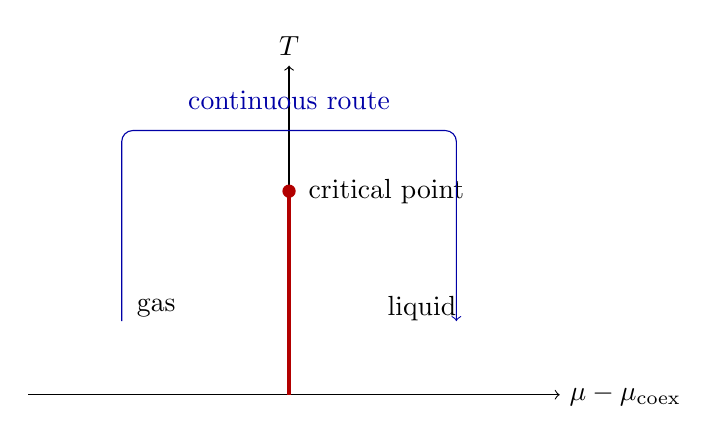
\begin{tikzpicture}[x=1.25cm,y=1.1cm]
\draw[->] (-2.65,0) -- (2.75,0) node[right] {$\mu-\mu_{\rm coex}$};
\draw[->] (0,0) -- (0,3.8) node[above] {$T$};
\draw[very thick,red!70!black] (0,0) -- (0,2.35);
\fill[red!70!black] (0,2.35) circle (2.4pt);
\node[right] at (0.1,2.35) {critical point};
\node at (-1.35,1.0) {gas};
\node at (1.35,1.0) {liquid};
\draw[->,blue!65!black,rounded corners]
 (-1.7,0.85) -- (-1.7,3.05) -- (1.7,3.05) -- (1.7,0.85);
\node[blue!65!black] at (0,3.4) {continuous route};
\end{tikzpicture}
\caption{Chất lỏng và khí là những pha phân biệt ở dưới điểm cuối, nhưng không có biên kỳ dị nào ngăn cách chúng trong vùng siêu tới hạn.}
\label{fig:liquid-gas-plane}
\end{figure}

Điều này xác định đường sôi quen thuộc. Ở áp suất cố định, nung nóng một chất lỏng cho đến khi nó đi qua đường cùng tồn tại sẽ gây ra sự sôi. Ở nhiệt độ cố định, thay đổi áp suất hoặc thế hóa học có thể đi qua cùng biên đó. Hơi quá nhiệt hoặc chất lỏng siêu nguội là sự tiếp diễn siêu bền vượt ra ngoài trạng thái cùng tồn tại cân bằng; việc mô tả thời gian sống của nó đòi hỏi động lực học tạo mầm, vốn nằm ngoài phép xây dựng cân bằng này.

\begin{classroomqa}
\audiencequestion{Hơi nước quá nhiệt có được biểu diễn trong giản đồ pha này không?}
\lecturerresponse{Giản đồ cân bằng xác định biên cùng tồn tại. Một trạng thái quá nhiệt hoặc quá bão hòa là siêu bền: nó tạm thời tồn tại ở phía không đúng vì việc hình thành một giọt tới hạn có chi phí năng lượng tự do của mặt phân cách. Sự tinh chỉnh động học đó không được tính ở đây. \lecturetimestamp{01:12:19--01:12:29}}
\end{classroomqa}

\begin{classroomqa}
\audiencequestion{Người ta thay đổi thế hóa học trong một chất lưu thông thường bằng cách nào?}
\lecturerresponse{Hộp giếng thế là cách điều khiển lý thuyết rõ ràng nhất. Trong phòng thí nghiệm, người ta thường thay đổi áp suất, thể tích, hoặc sự tiếp xúc với một bể chứa; khi đó nhiệt động lực học chuyển các điều khiển ấy thành sự thay đổi của thế hóa học. \lecturetimestamp{01:12:30--01:13:59}}
\end{classroomqa}

\begin{classroomqa}
\audiencequestion{Khi mật độ thay đổi, có phải ta đang thay đổi thế phân tử \(J\) không?}
\lecturerresponse{Không. Đối với một chất cố định, \(J\) biểu diễn lực hút tầm ngắn và giữ nguyên trong mô hình này. Thay đổi \(\mu\) làm thay đổi số ô mạng bị chiếm và do đó là phân bố các khoảng cách liên phân tử. Thay đổi \(J\) sẽ có nghĩa là thay đổi bản chất vi mô của chất hoặc của tương tác. \lecturetimestamp{01:14:50--01:15:41}}
\end{classroomqa}

\begin{classroomqa}
\audiencequestion{Nhiệt độ tới hạn có phải chính là điểm sôi thông thường không?}
\lecturerresponse{Không. Một điểm sôi được xác định tại một áp suất đã chọn, nên nó dịch chuyển dọc theo đường cùng tồn tại khi áp suất thay đổi. Nhiệt độ tới hạn là điểm cuối duy nhất mà ở phía trên nó, chất lỏng và khí không còn bị ngăn cách bởi một biên pha. Áp suất chưa được suy ra tường minh trong mô tả khí mạng này. \lecturetimestamp{01:15:42--01:17:02}}
\end{classroomqa}

Bây giờ có thể phát biểu kết quả trung tâm. Nam châm Ising và khí mạng không chỉ đơn thuần cho ra các giản đồ tương tự. Sau một phép đổi biến và tham số, chúng có chung một hàm phân hoạch. Mọi tính chất nhiệt động kỳ dị ở một phía đều có một đối ứng ở phía kia:
\begin{equation}
\begin{array}{c|c}
\text{Ising magnet} & \text{lattice gas}\\ \hline
\sigma_i=\pm1 & n_i=0,1\\
m=\expect{\sigma} & \rho=(1+m)/2\\
h & \mu=-(4dJ+2h)\\
\text{aligned exchange} & \text{nearest-neighbor attraction}\\
h=0,\ T<T_c & \text{liquid--gas coexistence}\\
(T_c,0) & \text{critical endpoint}
\end{array}
\label{eq:ising-fluid-dictionary}
\end{equation}

\section{Các số mũ tới hạn và tính phổ quát}

Gần một điểm tới hạn, các đại lượng nhiệt động thường phát sinh các kỳ dị theo luật lũy thừa. Với nhiệt độ rút gọn
\begin{equation}
t=\frac{T-T_c}{T_c},
\end{equation}
ta viết, một cách sơ đồ,
\begin{equation}
m\sim(-t)^{\beta_{\rm crit}},
\qquad
\chi\sim |t|^{-\gamma},
\qquad
\xi\sim |t|^{-\nu}.
\label{eq:critical-exponents}
\end{equation}
Ở đây \(\beta_{\rm crit}\) là một số mũ tới hạn, không phải nhiệt độ nghịch đảo. Lý thuyết trường trung bình cho \(\beta_{\rm crit}=1/2\), nhưng các thăng giáng làm thay đổi các số mũ ở dưới số chiều tới hạn trên.

Các số mũ không nhất thiết là số nguyên. Chúng cũng không nhất thiết đều là số vô tỉ: mô hình Ising hai chiều nổi tiếng có một số số mũ hữu tỉ chính xác, trong khi các giá trị của Ising ba chiều là những con số không tầm thường được xác định với độ chính xác cao bằng lý thuyết và tính toán. Bài học vững chắc là nói chung các số mũ không được ấn định bởi phân tích thứ nguyên sơ cấp.

Ấn tượng hơn nữa, các chi tiết vi mô thường không ấn định chúng. Các hệ có cùng số chiều không gian, cùng đối xứng của tham số trật tự, và các tương tác đủ tầm ngắn có thể chảy về cùng một lý thuyết tới hạn ở thang khoảng cách lớn. Chúng thuộc cùng một \emph{lớp phổ quát}. Một nam châm đơn trục và một điểm cuối lỏng--khí thông thường đều có một tham số trật tự vô hướng duy nhất và cùng thuộc lớp phổ quát Ising trong cùng số chiều.

\begin{classroomqa}
\audiencequestion{Các lớp phổ quát có phải là một danh sách hữu hạn hoặc rời rạc không?}
\lecturerresponse{Có nhiều lớp, được tổ chức theo số chiều, các đối xứng, các định luật bảo toàn, tầm của tương tác, và những dữ liệu khoảng cách lớn khác. Trong nhiều trường hợp quen thuộc, các điểm bất động và các bộ số mũ là rời rạc, nhưng cũng có những hệ có các số mũ biến thiên liên tục. Điều có thể khẳng định một cách an toàn không phải là danh mục ấy hữu hạn; mà là nhiều hệ khác nhau ở mức vi mô lại chia sẻ cùng một dữ liệu khoảng cách lớn. \lecturetimestamp{01:18:50--01:19:38}}
\end{classroomqa}

\begin{classroomqa}
\audiencequestion{Nếu chất lỏng và khí cùng tồn tại, cái gì ngăn cách chúng trong một bình chứa thực?}
\lecturerresponse{Một mặt phân cách. Sức căng bề mặt làm tăng năng lượng khi diện tích mặt phân cách tăng, còn trọng lực tạo ra một gradient thế hóa học theo phương thẳng đứng và thường đặt chất lỏng đậm đặc hơn ở dưới khí. Khi có thể bỏ qua trọng lực, hình học được chi phối trực tiếp hơn bởi sức căng bề mặt và các điều kiện biên. \lecturetimestamp{01:19:40--01:21:18}}
\end{classroomqa}

\begin{classroomqa}
\audiencequestion{Nhiệt hóa hơi nằm ở đâu trong bức tranh này?}
\lecturerresponse{Ở dưới điểm tới hạn, việc đi qua đường cùng tồn tại bậc một nói chung thường kèm theo ẩn nhiệt. Nhiệt hóa hơi tiến về không khi tiến gần điểm cuối tới hạn vì tại đó hai pha trở nên đồng nhất. Bài giảng này thiết lập cấu trúc pha nhưng không tính ẩn nhiệt. \lecturetimestamp{01:21:19--01:22:18}}
\end{classroomqa}

\begin{classroomqa}
\audiencequestion{Có thể dùng một chuyển pha như một đầu dò nhạy, chẳng hạn với một thiết bị siêu dẫn, không?}
\lecturerresponse{Có. Gần một chuyển pha, một nhiễu loạn nhỏ có thể tạo ra một đáp ứng lớn hoặc kích hoạt một sự đổi trạng thái. Các đầu dò thực tế khai thác độ nhạy ấy, mặc dù tham số trật tự và động lực học liên quan có thể khác với ví dụ Ising. \lecturetimestamp{01:22:19--01:24:05}}
\end{classroomqa}

Đến đây khóa học cơ học thống kê đã hoàn tất. Hành trình bắt đầu với entropy và cân bằng, đi qua hàm phân hoạch và chất khí, rồi kết thúc bằng việc chỉ ra rằng một nam châm và một chất lưu có thể là hai mô tả của cùng một hiện tượng tới hạn.

\section{Thảo luận sau bài giảng: sự tinh chỉnh và chọn lọc}

Sau khi bài giảng chính thức kết thúc, cuộc trao đổi tiếp tục thêm khoảng 40 phút. Phần này đáng được lưu lại, nhưng không nên nhầm nó với phép suy diễn ở trên. Chủ đề không còn là khí mạng nữa. Đó là logic của sự tinh chỉnh và việc sử dụng thận trọng chọn lọc vị nhân trong vũ trụ học.

\subsection{Những số nhỏ không tự động là các giá trị tinh chỉnh}

Không có một câu duy nhất nào giải quyết được mọi cách dùng của cụm \emph{nguyên lý vị nhân}. Điểm khởi đầu hữu ích mang tính thao tác: khi một lý thuyết cho phép nhiều môi trường được hiện thực hóa, các quan sát bị điều kiện hóa bởi sự kiện rằng người quan sát chỉ có thể nảy sinh trong một số môi trường ấy. Phát biểu có điều kiện đó có thể là hợp lý. Nó trở nên rỗng nếu được viện dẫn mà không có một tập hợp, một điều kiện chọn lọc, hoặc một cơ chế khiến các khả năng thay thế có ý nghĩa vật lý.

Trước khi xét đến chọn lọc, ta phải phân biệt một tham số nhỏ với một tham số tinh chỉnh. Một con số có thể nhỏ vì một cơ chế động lực học ổn định đẩy nó về một giá trị đặc biệt. Tinh chỉnh có nghĩa là giá trị được quan sát dường như đòi hỏi một sự cân bằng chính xác đến khác thường giữa các đóng góp vốn dĩ độc lập, mà không có cơ chế phục hồi hay đối xứng nào đã biết bảo vệ sự cân bằng đó.

\begin{classroomqa}
\audiencequestion{Nguyên lý vị nhân có thể được phát biểu một cách chặt chẽ không?}
\lecturerresponse{Cách dùng có thể biện hộ của nó mang tính điều kiện chứ không huyền bí: nếu nhiều môi trường được hiện thực hóa về mặt vật lý có các tham số khác nhau, thì những môi trường mà các sinh thể như chúng ta quan sát được sẽ được rút ra từ tập con tương thích với người quan sát. Điều đó tự nó không tạo ra các môi trường ấy hoặc gán xác suất cho chúng; những nhiệm vụ đó thuộc về vật lý nền tảng. \lecturetimestamp{01:25:45--01:26:13}}
\end{classroomqa}

Hằng số vũ trụ là ví dụ tạo động lực. Độ lớn quan sát được của nó nhỏ phi thường so với các đóng góp ngây thơ của lý thuyết trường lượng tử vào năng lượng chân không. Khó khăn không chỉ đơn thuần là con số cuối cùng nhỏ. Mà là dường như nhiều hạng lớn phải triệt tiêu nhau với độ chính xác cực kỳ cao, trong khi không có cơ chế hồi tiếp năng lượng thấp nào được chấp nhận để điều chỉnh kết quả về phía giá trị quan sát được.

\subsection{Khí cầu và tàu ngầm}

Hai ví dụ về lực nổi làm rõ sự phân biệt này. Một khí cầu lơ lửng ở độ cao mà tại đó mật độ trung bình của nó bằng mật độ của không khí xung quanh. Mật độ không khí giảm theo độ cao. Nếu khí cầu bay lên, không khí bên ngoài trở nên loãng hơn và khí cầu có xu hướng hạ xuống; nếu nó hạ xuống, không khí bên ngoài trở nên đặc hơn và khí cầu có xu hướng bay lên. Sự khớp mật độ ấy có thể tinh tế về mặt số trị, nhưng gradient khí quyển cung cấp hồi tiếp phục hồi. Trạng thái cân bằng được giải thích bằng động lực học.

Một tàu ngầm có lực nổi trung hòa trong nước gần như không nén được thì khác. Mật độ của nước thay đổi rất ít theo độ sâu. Nếu mật độ trung bình của tàu ngầm tình cờ bằng mật độ của nước xung quanh, không có cơ chế phục hồi phụ thuộc độ sâu nào tương đương để giải thích sự bằng nhau đó. Một sai lệch rất nhỏ cũng khiến nó nổi lên hoặc chìm xuống. Để đạt được lực nổi trung hòa cần điều chỉnh chính xác vật dằn và các thành phần bên trong. Khi đó phần dư nhỏ còn lại là một sự tinh chỉnh, trừ phi có hệ điều khiển hoặc cơ chế thiết kế nào đó giải thích cho nó.

\begin{figure}[ht]
\centering
\resizebox{\linewidth}{!}{%
\begin{tikzpicture}[>=Latex]
\begin{scope}[xshift=-3.8cm]
\shade[top color=blue!5,bottom color=blue!28] (-2.5,-2.2) rectangle (2.5,2.2);
\draw[very thick,rounded corners=18pt,fill=yellow!35]
  (-1.15,0) ellipse (1.15 and 0.55);
\draw[thick] (0,-0.55) -- (0,-1.05);
\draw[thick,fill=gray!20] (-0.45,-1.05) rectangle (0.45,-1.38);
\draw[->,red!70!black,thick] (1.65,1.45) -- (1.65,0.55)
 node[midway,right] {restoring};
\draw[->,red!70!black,thick] (-1.65,-1.45) -- (-1.65,-0.55)
 node[midway,left] {restoring};
\node at (0,2.55) {\textbf{Blimp: density gradient}};
\node[align=center] at (0,-2.75) {displacement changes\\the buoyant imbalance};
\end{scope}
\begin{scope}[xshift=3.8cm]
\shade[top color=cyan!10,bottom color=blue!45] (-2.5,-2.2) rectangle (2.5,2.2);
\draw[very thick,fill=gray!35,rounded corners=12pt]
  (-1.45,-0.25) -- (1.1,-0.25) arc (-90:90:0.38)
  -- (-1.45,0.51) -- cycle;
\draw[thick] (-0.25,0.51) -- (-0.25,0.85) -- (0.35,0.85) -- (0.35,0.51);
\draw[->,red!70!black,thick] (1.65,0.15) -- (1.65,1.35)
 node[midway,right] {rise};
\draw[->,red!70!black,thick] (-1.65,0.15) -- (-1.65,-1.35)
 node[midway,left] {sink};
\node at (0,2.55) {\textbf{Submarine: nearly uniform density}};
\node[align=center] at (0,-2.75) {no depth-dependent feedback\\protects neutral buoyancy};
\end{scope}
\end{tikzpicture}
}
\caption{Một phần dư nhỏ có thể ổn định về mặt động lực học hoặc thực sự là do tinh chỉnh. Khí cầu có hồi tiếp phục hồi; tàu ngầm lý tưởng hóa đòi hỏi mật độ trung bình của nó phải được điều chỉnh cho bằng mật độ của nước.}
\label{fig:blimp-submarine}
\end{figure}

\begin{classroomqa}
\audiencequestion{Vì sao thủy thủ đoàn tàu ngầm phải đòi hỏi một lời giải thích nếu quan sát thấy lực nổi trung hòa?}
\lecturerresponse{Bởi vì, nếu không có cơ chế điều khiển vật dằn, thì cả đối xứng lẫn hồi tiếp môi trường đều không bảo vệ sự bằng nhau của hai mật độ độc lập. Vấn đề không phải là liệu sự bằng nhau đó có khả hữu về mặt logic hay không, mà là vì sao hệ lại nằm trong một vùng hẹp đến như vậy của không gian tham số của nó. \lecturetimestamp{01:35:05--01:36:25}}
\end{classroomqa}

\subsection{Nhiều miền và quan sát có điều kiện}

Bây giờ hãy tưởng tượng một quá trình tạo ra một số lượng khổng lồ tàu ngầm với nhiều mật độ trung bình khác nhau. Phần lớn chìm hoặc nổi lên; chỉ một phần rất nhỏ còn tồn tại lâu dài trong dải có thể cư trú giữa mặt nước và đáy. Một người quan sát, vốn nhất thiết phải sống trong một trong những tàu ngầm còn tồn tại ấy, không nên ngạc nhiên khi đo được trạng thái gần như nổi trung hòa. Quan sát này được chọn lọc bởi điều kiện cần để người quan sát có mặt.

Lập luận này cần hai thành phần:
\begin{enumerate}
\item một quá trình vật lý thực sự hiện thực hóa nhiều khả thể, chứ không phải những khả thể chỉ tồn tại trong tưởng tượng;
\item một điều kiện chọn lọc giải thích vì sao các quan sát chỉ được thực hiện trong một tập con bị hạn chế.
\end{enumerate}
Chọn lọc không thay thế cơ chế tạo ra. Nó làm thay đổi xác suất có điều kiện của điều mà một người quan sát đo được một khi tập hợp đã tồn tại.

\begin{classroomqa}
\audiencequestion{Có phải lập luận này chỉ đơn thuần là rằng những điều khó xảy ra vẫn xảy ra ở đâu đó trong một mẫu đủ lớn?}
\lecturerresponse{Đó mới chỉ là nửa đầu. Nửa còn lại là điều kiện hóa quan sát: người quan sát không được lấy mẫu đồng đều từ mọi miền mà chỉ từ những miền nơi sự tồn tại của họ là khả dĩ. Một đề xuất hoàn chỉnh vẫn cần một độ đo trên các miền và một mô tả vật lý về cách chúng được tạo ra. \lecturetimestamp{01:39:19--01:40:36}}
\end{classroomqa}

Áp dụng cho năng lượng chân không, một hằng số vũ trụ âm lớn có thể khiến một vũ trụ tái co sụp quá nhanh, trong khi một giá trị dương đủ lớn có thể ngăn vật chất ngưng tụ thành các thiên hà. Giá trị quan sát được nằm trong khoảng hẹp tương thích với cấu trúc tồn tại lâu dài. Điều này cung cấp một điều kiện chọn lọc khả dĩ, chứ không phải một phép suy ra phân bố của các hằng số vũ trụ.

Lý thuyết trường lượng tử còn làm nảy sinh bài toán tinh chỉnh: các đóng góp chân không từ những trường và thang khác nhau, xét riêng lẻ, đều lớn hơn rất nhiều so với phần dư quan sát được. Nếu những hạng đó triệt tiêu nhau gần như chính xác hoàn toàn, thì kết quả giống với tàu ngầm được cân bằng cẩn thận hơn là khí cầu tự hiệu chỉnh. Phép loại suy này nhằm phơi bày vấn đề logic, chứ không cung cấp lời giải cho nó.

\begin{classroomqa}
\audiencequestion{Liệu những thay đổi của một tham số có thể được bù bởi những thay đổi của một số tham số khác không?}
\lecturerresponse{Có. Tập khả thi không nhất thiết phải là một khoảng hẹp trên một trục; nó có thể là một mặt mỏng trong không gian tham số nhiều chiều. Những thay đổi tương quan có thể bảo toàn cấu trúc, nhưng khi đó câu hỏi trở thành vì sao các tham số được hiện thực hóa lại nằm gần mặt ấy và lý thuyết nền tảng gán cho nó độ đo nào. \lecturetimestamp{01:45:10--01:46:19}}
\end{classroomqa}

\begin{figure}[ht]
\centering
\begin{tikzpicture}[x=1.3cm,y=1.05cm,>=Latex]
\draw[->] (-3.2,0) -- (3.4,0) node[right] {$\lambda_1$};
\draw[->] (0,-2.5) -- (0,2.65) node[above] {$\lambda_2$};
\fill[gray!12] (-3,-2.25) rectangle (3.1,2.3);
\draw[very thick,blue!65!black]
 (-2.8,-1.55) .. controls (-1.3,-0.75) and (0.15,0.05) .. (2.85,1.55);
\draw[very thick,blue!25]
 (-2.8,-1.25) .. controls (-1.3,-0.45) and (0.15,0.35) .. (2.85,1.85);
\fill[blue!15,opacity=.65]
 (-2.8,-1.55) .. controls (-1.3,-0.75) and (0.15,0.05) .. (2.85,1.55)
 -- (2.85,1.85) .. controls (0.15,0.35) and (-1.3,-0.45) .. (-2.8,-1.25) -- cycle;
\node[blue!65!black,rotate=28] at (1.3,0.95) {viable band};
\foreach \x/\y in {-2.4/1.45,-1.7/-1.8,-0.9/1.8,0.3/-1.45,1.2/1.85,2.4/-0.8}
  \fill[red!65!black] (\x,\y) circle (2pt);
\fill[green!45!black] (0.55,0.58) circle (2.8pt);
\node[green!35!black,right] at (0.65,0.55) {observed domain};
\end{tikzpicture}
\caption{Với nhiều tham số, tính khả cư hoặc tính khả thi của cấu trúc có thể chiếm một dải tương quan mỏng thay vì một khoảng hẹp của một tham số duy nhất. Chọn lọc ràng buộc các quan sát vào dải đó nhưng không tạo ra phân bố tham số.}
\label{fig:viable-parameter-band}
\end{figure}

\subsection{Các đề xuất landscape và những bất định của chúng}

Một nguồn gốc được đề xuất cho các khả thể thay thế là một lý thuyết có nhiều trạng thái chân không giả bền, có thể được chiếm giữ trong những miền vũ trụ khác nhau. Các ý tưởng landscape của lý thuyết dây và các kịch bản lạm phát vĩnh cửu là những ví dụ, nhưng cách hiện thực hóa chi tiết và độ đo xác suất của chúng vẫn còn bất định. Bài giảng trình bày điều này như một khả năng, chứ không phải một sự kiện đã được xác lập.

Đối xứng sẽ là một cách giải thích theo lối thông thường hơn nếu nó buộc hằng số vũ trụ triệt tiêu đúng bằng không. Khó khăn là sự giãn nở gia tốc được quan sát tương ứng với một giá trị nhỏ nhưng khác không. Một cơ chế tự nhiên cho đúng bằng không không tự động giải thích được một phần dư rất nhỏ; việc phá vỡ đối xứng có thể chỉ đơn giản là tái đưa sự tinh chỉnh trở lại. Hình ảnh chiếc tàu ngầm lại xuất hiện ở đây: một sợi dây có thể giữ nó ở độ sâu đã chọn, nhưng khi đó sợi dây mới là cơ chế cần được xác định thay vì bị mặc nhiên giả định.

\begin{classroomqa}
\audiencequestion{Việc đo một tham số với độ chính xác rất cao có vi phạm nguyên lý bất định không?}
\lecturerresponse{Không. Một hệ thức bất định áp dụng cho những cặp quan sát được không giao hoán đã được chỉ rõ. Một hằng số liên kết hoặc tham số chân không có thể có một giá trị được xác định sắc nét mà không phải là đại lượng liên hợp chính tắc của một quan sát được không được kiểm soát. Bản thân độ chính xác không phải là một nghịch lý của nguyên lý bất định. \lecturetimestamp{01:49:21--01:49:36}}
\end{classroomqa}

\begin{classroomqa}
\audiencequestion{Lập luận nhân học có giải thích giá trị ấy không, hay chỉ đơn thuần nhắc lại rằng người quan sát cần nó?}
\lecturerresponse{Chỉ riêng chọn lọc không phải là một lời giải thích động lực học. Vai trò chính đáng của nó là làm thay đổi các xác suất có điều kiện trong một tập hợp được hiện thực hóa về mặt vật lý. Nếu dùng nó mà không có một tập hợp, một độ đo, hoặc các hệ quả có thể kiểm nghiệm, nó có nguy cơ trở thành một cái nhãn hơn là một lời giải thích. \lecturetimestamp{01:49:37--01:50:21}}
\end{classroomqa}

\subsection{Những sự trùng hợp mức độ vừa phải trong vật lý hạt}

Không phải mọi tham số liên quan đến sự sống đều được tinh chỉnh đến cùng một mức độ phi thường. Vật chất thông thường phụ thuộc vào photon, electron, các quark nhẹ và tương tác mạnh; neutrino ảnh hưởng đến vũ trụ học nhưng không phải là tác nhân liên kết trực tiếp của các nguyên tử. Độ chênh khối lượng proton--neutron đặc biệt hệ trọng. Vì neutron hơi nặng hơn proton, các neutron cô lập có thể phân rã và hydro thông thường là bền. Đảo ngược thứ tự ấy một lượng đủ lớn sẽ làm biến đổi căn bản hóa học hạt nhân.

Khối lượng electron và hằng số cấu trúc tinh cũng xác định kích thước nguyên tử và năng lượng liên kết. Thay đổi chúng một cách đáng kể sẽ làm thay đổi hóa học. Đó là những phát biểu về độ nhạy có ý nghĩa, nhưng không nên thổi phồng thành khẳng định rằng mọi biến thiên nhỏ đều cấm mọi dạng phức tạp có thể hình dung được. So với bài toán hằng số vũ trụ, nhiều sự trùng hợp như vậy là mức độ vừa phải và có tương quan với các tham số khác.

Vấn đề phân cấp gắn với thang điện yếu là một bài toán tính tự nhiên nổi bật khác: các đóng góp bức xạ có xu hướng làm cho khối lượng của một hạt vô hướng cơ bản nhạy với các thang cao, trừ phi được bảo vệ bởi cấu trúc bổ sung. Vị thế và cách diễn giải của nó khác với bài toán năng lượng chân không, và không nên rút gọn cái nào thành một khẩu hiệu.

\begin{classroomqa}
\audiencequestion{Việc thay đổi độ chênh khối lượng proton--neutron thực sự có ảnh hưởng đối với vật chất thông thường không?}
\lecturerresponse{Có. Thứ tự được quan sát cho phép hydro bền và chi phối tính bền beta của các hạt nhân. Những thay đổi vừa phải có thể sắp xếp lại độ phong phú hạt nhân và sự cháy sao. Một phân tích cẩn thận phải làm biến thiên các tham số liên đới một cách nhất quán, thay vì thay đổi một con số trong khi giữ cố định tất cả phần còn lại. \lecturetimestamp{01:51:47--01:53:08}}
\end{classroomqa}

\begin{classroomqa}
\audiencequestion{Khối lượng electron và hằng số cấu trúc tinh đóng những vai trò gì?}
\lecturerresponse{Chúng đặt ra các thang năng lượng và độ dài nguyên tử đặc trưng, một cách sơ đồ là \(E_{\rm atom}\sim \alpha^2m_e\) và \(a_0\sim(\alpha m_e)^{-1}\) trong đơn vị \(\hbar=c=1\). Những thay đổi lớn sẽ định hình lại hóa học, mặc dù miền khả thi chính xác là một câu hỏi nhiều chiều. \lecturetimestamp{01:53:09--01:54:12}}
\end{classroomqa}

\subsection{Bất đồng, sự phụ thuộc theo thời gian và các phép kiểm nghiệm}

Phần thảo luận chuyển ngắn gọn sang những phê phán đối với lạm phát và sang cách diễn giải dữ liệu vũ trụ học có độ chính xác cao. Bất đồng mang tính lịch sử ấy cần được trình bày đúng là một bất đồng, chứ không phải như thể đã được giải quyết bằng lời lẽ hùng biện. Lạm phát có những dự đoán hiện tượng học thành công và nhiều biến thể mô hình; các câu hỏi về điều kiện ban đầu, độ đo và khả năng kiểm định vẫn còn là những vấn đề đang được nghiên cứu tích cực. Dữ liệu ràng buộc các mô hình, nhưng không một lời viện dẫn thoáng qua nào tới một thí nghiệm có thể quyết định toàn bộ khuôn khổ đó.

\begin{classroomqa}
\audiencequestion{Liệu hằng số vũ trụ có thể biến thiên chậm theo thời gian thay vì là hằng số không?}
\lecturerresponse{Một trường năng lượng tối động lực học có thể tạo ra sự gia tốc phụ thuộc thời gian. Nó đưa vào một thế năng và các điều kiện ban đầu mà bản thân chúng cũng phải được giải thích, và các quan sát ràng buộc phương trình trạng thái phải gần với một hằng số vũ trụ. Trong phần thảo luận ở thời điểm bài giảng, không có bằng chứng nào đòi hỏi một sự biến thiên theo thời gian đáng kể. \lecturetimestamp{01:57:17--01:59:19}}
\end{classroomqa}

\begin{classroomqa}
\audiencequestion{Bản thân chọn lọc vị nhân có làm nảy sinh các vũ trụ hay các miền khác nhau không?}
\lecturerresponse{Không. Chọn lọc chỉ cho biết những miền đã được hiện thực hóa nào có thể chứa các quan sát viên; nó không tạo ra các miền ấy. Chúng phải được sinh ra bởi một cơ chế vũ trụ học riêng biệt, chẳng hạn các chuyển tiếp chân không trong một lịch sử lạm phát. \lecturetimestamp{01:59:20--01:59:42}}
\end{classroomqa}

Trật tự nhân quả phải luôn rõ ràng:
\begin{equation}
\begin{gathered}
\text{laws and initial conditions}\\[-0.15em]
\downarrow\\[-0.15em]
\text{physical environments}\\[-0.15em]
\downarrow\\[-0.15em]
\text{observers and observations}
\end{gathered}
\end{equation}
Các quan sát viên không vươn ngược trở lại để áp đặt các định luật. Việc điều kiện hóa xuất hiện khi ta hỏi một quan sát viên được chọn từ các môi trường đã được hiện thực hóa có khả năng sẽ đo được điều gì.

Vì thế, câu hỏi khoa học không phải là liệu ngôn ngữ ấy nghe có vẻ triết học, chính trị hay tôn giáo hay không. Mà là liệu đề xuất đó có một ensemble vật lý được xác định, một độ đo có thể tính được hoặc ít nhất cũng được ràng buộc, và những hệ quả có thể phân biệt nó với các phương án thay thế hay không. Các dấu hiệu khả dĩ đã được bàn đến đối với vũ trụ học đa chân không bao gồm các vết tích của va chạm giữa các miền bong bóng. Những tín hiệu như vậy khó được dự đoán một cách vững chắc, và trong phần thảo luận ở thời điểm bài giảng chưa có tín hiệu nào như thế được xác lập trong bức xạ nền vi sóng vũ trụ. Việc thiếu một phép kiểm nghiệm dễ dàng là một hạn chế nghiêm trọng, chứ không cho phép ta hoặc tuyên bố ý tưởng ấy là đúng, hoặc gạt bỏ vấn đề tinh chỉnh ở nền tảng.

\begin{classroomqa}
\audiencequestion{Điều gì sẽ biến lập luận chọn lọc này thành một lý thuyết khoa học?}
\lecturerresponse{Đề xuất ấy cần một cơ chế sinh ra các phương án thay thế, một độ đo xác suất hoặc một phương án thay thế được kiểm soát, và các hệ quả có thể quan sát được. Các dấu hiệu va chạm bong bóng là một hướng khả dĩ, nhưng sự vắng mặt hoặc tính mơ hồ của chúng cho thấy vấn đề khả năng kiểm định đòi hỏi đến mức nào. \lecturetimestamp{02:02:31--02:04:12}}
\end{classroomqa}

Phần trao đổi sau bài giảng kết thúc trên tinh thần chặt chẽ ấy. Sự tinh chỉnh là bằng chứng cho thấy có thể đang thiếu một lời giải thích. Đối xứng, sự điều chỉnh động lực học và chọn lọc theo môi trường là những cách giải thích ứng viên khác nhau về mặt logic. Chọn lọc có thể là hợp lý, nhưng chỉ như một thành phần của một lý giải vật lý mà các giả định và giới hạn của nó được nêu ra minh bạch.
